
\chapter{Organizing Committee}

\begin{description}

 \item[AB3C President]: Alan M Durham (USP)

\item[AB3C Vice President]: Ney Lemke (UNESP)

  
\item[AB3C Secretaries]:

\begin{itemize}
 \item Marcelo Brand\~ao (Unicamp) 
 \item  Fabr\'{\i}cio Martins Lopes  (UTFPR)
\end{itemize}

\item[AB3C Financial Department]:

\begin{itemize}
\item Priscila Grynberg (Embrapa)
\item Nicole Scherer (Fiocruz)
\end{itemize}


\item[Poster Session Organizers]:

\begin{itemize}
  \item Robson Francisco de Souza (USP)
\item Nicole Scherer (INCA)
\end{itemize}

 \item[Scientific Comitttee]:

  \begin{itemize}
    \item  Andr\'e Fujita (USP)
    \item  Andr\'e Yoshiaki Kashiwabara (UTFPR)
    \item Arthur Gri\"uuber (USP)
    \item Guilherme Targino Valente (Unesp)
    \item Katlin Brauer Massirer (UNICAMP)
    \item M\'arcio Dom (UFRGS)
    \item Maria Berenice Reynaud Steffens (UFPR)
    \item Robson Francisco de Souza (USP)
  \end{itemize}
\item[Highlight Track Organizer]:
\begin{itemize}
\item Priscila Grynberg (Embrapa)
\item Nicole Scherer (Fiocruz)
\end{itemize} 
\end{description}


\newpage
\chapter{Introduction}
The Brazilian Association of Bioinformatics and Computational Biology (AB3C) is
a scientific society funded in July 12th 2004.
Since its creation, AB3C has been responsible for the annual conference entitled
''X-Meeting'' which is the main Bioinformatics and Computation Biology event in
Brazil. This year its 13th edition occurred in S\~ao Pedro on October
\nth{4}-\nth{6} .

	
Bioinformatics is now a strategic area for Brazil and all Latin America and,
therefore, it is also strategic to the development of Science, Technology and
Economy. The X-Meeting is a Brazilian event with international reach which has
an average of 400 participants. The Conference is an opportunity for students,
researchers and companies to interact and difuse knowledge. The AB3C has been a
pioneer society in the field of Bioinformatics in Brazil and we have a history
of ten past very productive meetings.

\begin{figure}[h]
    \begin{center}
  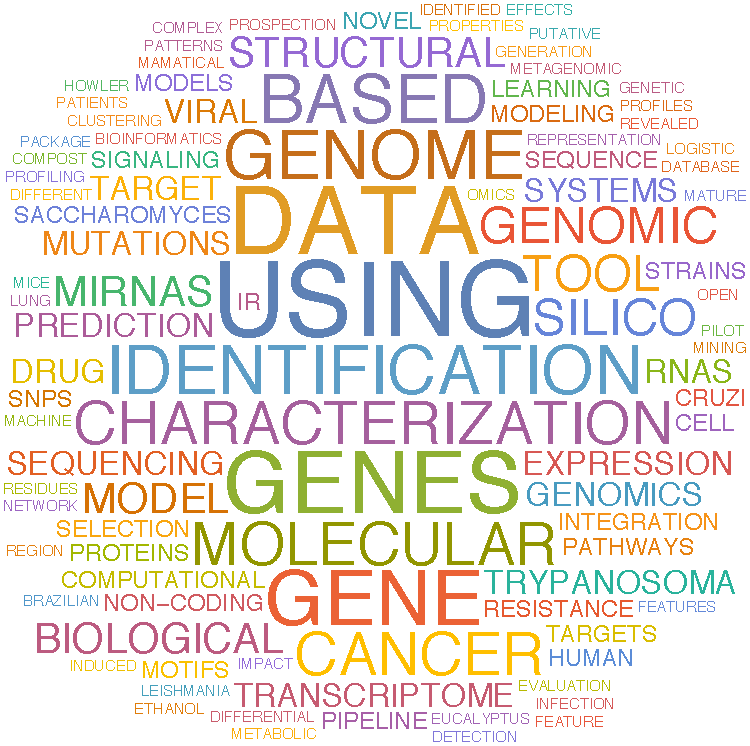
\includegraphics[scale=0.7]{wordcloud}
\end{center}
\caption{Word Cloud for the words used on the Conference Papers Titles}
\end{figure}


\begin{landscape}
\begin{figure}[h]
    \begin{center}
  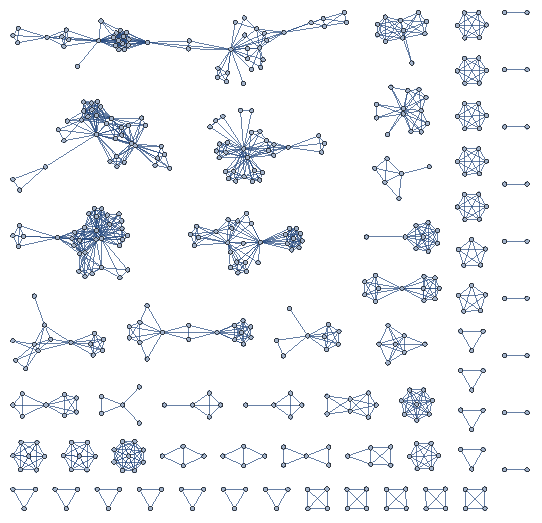
\includegraphics[scale=1.5,angle=0]{grafo}
\end{center}
\caption{Graph representing the network of collaborations of the X-meeting 2016. An interactive 
version of this graph can be seen at \url{https://neylemke.github.io/assets/grafo.html}}
\end{figure}
\end{landscape}
